%%%%%%%%%%%%%%%%%%%%%%%%%%%%%%%%%%%%%%%%%
% Arsclassica Article
% LaTeX Template
% Version 1.1 (1/8/17)
%
% This template has been downloaded from:
% http://www.LaTeXTemplates.com
%
% Original author:
% Lorenzo Pantieri (http://www.lorenzopantieri.net) with extensive modifications by:
% Vel (vel@latextemplates.com)
%
% License:
% CC BY-NC-SA 3.0 (http://creativecommons.org/licenses/by-nc-sa/3.0/)
%
%%%%%%%%%%%%%%%%%%%%%%%%%%%%%%%%%%%%%%%%%

%----------------------------------------------------------------------------------------
%	PACKAGES AND OTHER DOCUMENT CONFIGURATIONS
%----------------------------------------------------------------------------------------

\documentclass[
10pt, % Main document font size
a4paper, % Paper type, use ``letterpaper'' for US Letter paper
oneside, % One page layout (no page indentation)
%twoside, % Two page layout (page indentation for binding and different headers)
headinclude,footinclude, % Extra spacing for the header and footer
BCOR5mm, % Binding correction
]{scrartcl}

%%%%%%%%%%%%%%%%%%%%%%%%%%%%%%%%%%%%%%%%%
% Arsclassica Article
% Structure Specification File
%
% This file has been downloaded from:
% http://www.LaTeXTemplates.com
%
% Original author:
% Lorenzo Pantieri (http://www.lorenzopantieri.net) with extensive modifications by:
% Vel (vel@latextemplates.com)
%
% License:
% CC BY-NC-SA 3.0 (http://creativecommons.org/licenses/by-nc-sa/3.0/)
%
%%%%%%%%%%%%%%%%%%%%%%%%%%%%%%%%%%%%%%%%%

%----------------------------------------------------------------------------------------
%	REQUIRED PACKAGES
%----------------------------------------------------------------------------------------

\usepackage[
nochapters, % Turn off chapters since this is an article        
beramono, % Use the Bera Mono font for monospaced text (\texttt)
eulermath,% Use the Euler font for mathematics
pdfspacing, % Makes use of pdftex’ letter spacing capabilities via the microtype package
dottedtoc % Dotted lines leading to the page numbers in the table of contents
]{classicthesis} % The layout is based on the Classic Thesis style

\usepackage{arsclassica} % Modifies the Classic Thesis package

\usepackage[T1]{fontenc} % Use 8-bit encoding that has 256 glyphs

\usepackage[utf8]{inputenc} % Required for including letters with accents

\usepackage{graphicx} % Required for including images
\graphicspath{{Figures/}} % Set the default folder for images

\usepackage{enumitem} % Required for manipulating the whitespace between and within lists

\usepackage{lipsum} % Used for inserting dummy 'Lorem ipsum' text into the template

\usepackage{subfig} % Required for creating figures with multiple parts (subfigures)

\usepackage{amsmath,amssymb,amsthm} % For including math equations, theorems, symbols, etc

\usepackage{varioref} % More descriptive referencing

\usepackage[spanish]{babel} % spanish

%----------------------------------------------------------------------------------------
%	THEOREM STYLES
%---------------------------------------------------------------------------------------

\theoremstyle{definition} % Define theorem styles here based on the definition style (used for definitions and examples)
\newtheorem{definition}{Definition}

\theoremstyle{plain} % Define theorem styles here based on the plain style (used for theorems, lemmas, propositions)
\newtheorem{theorem}{Theorem}

\theoremstyle{remark} % Define theorem styles here based on the remark style (used for remarks and notes)

%----------------------------------------------------------------------------------------
%	HYPERLINKS
%---------------------------------------------------------------------------------------

\hypersetup{
%draft, % Uncomment to remove all links (useful for printing in black and white)
colorlinks=true, breaklinks=true, bookmarks=true,bookmarksnumbered,
urlcolor=webbrown, linkcolor=RoyalBlue, citecolor=webgreen, % Link colors
pdftitle={}, % PDF title
pdfauthor={\textcopyright}, % PDF Author
pdfsubject={}, % PDF Subject
pdfkeywords={}, % PDF Keywords
pdfcreator={pdfLaTeX}, % PDF Creator
pdfproducer={LaTeX with hyperref and ClassicThesis} % PDF producer
} % Include the structure.tex file which specified the document structure and layout

\hyphenation{Fortran hy-phen-ation} % Specify custom hyphenation points in words with dashes where you would like hyphenation to occur, or alternatively, don't put any dashes in a word to stop hyphenation altogether

%----------------------------------------------------------------------------------------
%	TITLE AND AUTHOR(S)
%----------------------------------------------------------------------------------------

\title{\normalfont\spacedallcaps{Biología y Computación}} % The article title

%\subtitle{Subtitle} % Uncomment to display a subtitle

\author{\spacedlowsmallcaps{José Antonio Pereiro Morejón\textsuperscript{1}*}} % The article author(s) - author affiliations need to be specified in the AUTHOR AFFILIATIONS block

% \date{\today} % An optional date to appear under the author(s)

%----------------------------------------------------------------------------------------

\begin{document}

%----------------------------------------------------------------------------------------
%	HEADERS
%----------------------------------------------------------------------------------------

\lehead{\mbox{\llap{\small\thepage\kern1em\color{halfgray} \vline}\color{halfgray}\hspace{0.5em}\rightmark\hfil}} % The header style

\pagestyle{scrheadings} % Enable the headers specified in this block

%----------------------------------------------------------------------------------------
%	TABLE OF CONTENTS & LISTS OF FIGURES AND TABLES
%----------------------------------------------------------------------------------------

\maketitle % Print the title/author/date block

\setcounter{tocdepth}{2} % Set the depth of the table of contents to show sections and subsections only

\tableofcontents % Print the table of contents

%----------------------------------------------------------------------------------------
%	AUTHOR AFFILIATIONS
%----------------------------------------------------------------------------------------

\let\thefootnote\relax\footnotetext{\textsuperscript{1} \textit{Grupo de Computación, Facultad de Biología, Universidad de la Habana}}
\let\thefootnote\relax\footnotetext{* \textit{apereiro@fbio.uh.cu}}

% ----------------------------------------------------------------------------------------
%   CONTENT
% ----------------------------------------------------------------------------------------

\section{Introducción}
 
Al ser esta la primera asignatura en la carrera con carácter explícitamente computacional, hemos querido comenzar agregando un poco de contexto sobre la relación existente entre la Biología y la Computación.
Para ello, haremos una revisión muy breve sobre la historia de cómo la primera ha ido encontrando en esta última una herramienta cada vez más útil, incluso imprescindible, a la hora de resolver las cuestiones fundamentales en el estudio de la vida.
En su elaboración, el mayor reto al que nos enfrentamos es la diversidad de temas de interés.
La Biología es una ciencia muy amplia, que va desde los estudios más holísticos en la ecología y la conservación, hasta los más reduccionistas como la caracterización de una proteína.
Para cada una de estas áreas se pudiera hacer un relato independiente pero en casi todos encontraríamos un patrón similar.
La fracción de cualquier estudio biológico dependiente de las habilidades computacionales del investigador ha ido creciendo sostenidamente; ya sea durante la recolección de los datos, su análisis, su almacenamiento o su publicación \cite{gauthierBriefHistoryBioinformatics2019, cameronBriefHistorySynthetic2014}.
 
 
Por problemas de tiempo, y aceptando que dejaremos fuera muchos casos interesantes, en este documento nos centraremos en una historia en particular: el desarrollo y consolidación del Dogma Central de la Biología Molecular.
La justificación de nuestra selección es que dicho principio es uno de los conceptos fundamentales de la Biología moderna y encuentra aplicación en todas las áreas de la misma.
A grandes rasgos, este establece la popular noción de que en los sistemas vivos el flujo de información comienza típicamente por la secuencia de ADN (ácido desoxirribonucleico) y luego se ramifica escalonadamente por varios niveles.
Otro rasgo importante es que este proceso es unidireccional.
O sea, los cambios fenotípicos no se propagan hacia la cumbre de la jerarquía afectando a la secuencia de ADN \cite{crickCentralDogmaMolecular1970}.
Posteriormente profundizaremos más sobre el tema pero por ahora, comenzaremos un poco antes de que todo ese conocimiento se estableciera.


\section{Primera mitad del siglo XX}

% 5
Es increíble lo mucho que la ciencia ha avanzado en los últimos 120 años.
Como referencia, tengan en cuenta que al tiempo que Albert Einstein cursaba sus estudios universitarios todavía había un fuerte debate en la comunidad científica sobre lo que hoy asumimos como una verdad elemental: la materia está compuesta por átomos.
De hecho, en 1905 el propio Albert Einstein contribuyó al debate tratando de responder algo tan básico como: ¿de qué tamaño son los átomos? \cite{einsteinEinsteinMiraculousYear2021}.
Con el establecimiento de la teoría atómica y el posterior desarrollo de las Mecánicas Cuánticas y Estadísticas, se consolidaron y extendieron los resultados de otras ciencias más tradicionales como la Química y la Termodinámica.
Paralelo, en la Biología comienzan a enraizar corrientes que describen la vida como un proceso químico-físico, por ejemplo, la Bioquímica y la Biología Molecular.
Estas ciencias definen a las células como un pequeño reactor químico compuesto principalmente de agua y de un grupo de compuestos orgánicos: los carbohidratos, las proteínas, los ácidos nucleicos y los lípidos.

% 5
Aunque se progresaba sostenidamente, estos pudieran ser considerados todavía ``tiempos oscuros'' para la Biología.
Por ejemplo, resultados como que algunas proteínas tienen capacidad enzimática no fueron establecidos hasta 1926 \cite{sumnerISOLATIONCRYSTALLIZATIONENZYME1926}.
Además, otras preguntas fundamentales seguían abiertas.
A pesar que las teorías de la Herencia y Evolución estaban ya acompañadas de evidencias experimentales sólidas, como las aportadas por los registros fósiles, la Biología Comparada y experimentos de cruzamiento \cite{darwinOriginSpeciesMeans1859, abbottExperimentsPlantHybrids2016a}, sus bases moleculares seguían siendo un misterio.
 
% 5
El descubrimiento de que el ADN es el portador de la información genética fue uno de los logros más importantes de la Biología Molecular durante la década de 1950.
Para nada este fue un tema libre de controversias, muchos investigadores apostaban por las proteínas como el mejor candidato \cite{griffithsIntroductionGeneticAnalysis2006}.
Esto se debía a que para la época, el ADN era visto solo como una ``aburrida'' sustancia constituida por grandes cantidades de cuatro subunidades diferentes (bases nitrogenadas), las cuales se agrupaban en pares debido a que se encontraban en igual proporsión.
Había discusiones sobre si una sustancia tan simple químicamente era capaz de encerrar la complejidad necesaria para describir a un organismo completo.
Las proteínas, por otro lado, son más diversas al estar compuestas por veinte subunidades (aminoácidos) y hay miles diferentes en cada célula.
Esta discusión fue concluyendo ante los resultados de una serie de experimentos claves.
 
\begin{figure}[bb]
   \centering
   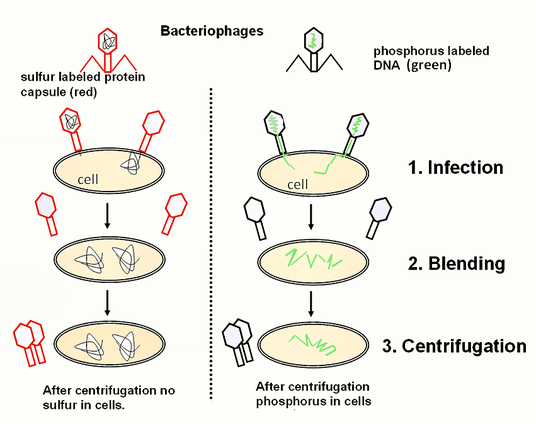
\includegraphics[width=0.6\columnwidth]{images/Martha_Chase_and_Alfred_Hershey_Experiment.png}
   \caption{(\textit{Figura en inglés}) Esquema del experimento de Martha Chase y Alfred Hershey. Más detalles en el texto principal. Fuente \cite{wiki:Alfred_Hershey_and_Martha_Chase_Experiment}}
   \label{fig:Martha_and_Hershey_Experiment}
\end{figure}

% 4
En 1944, ya se había observado que el ADN extraído de una cepa de bacteria podía transferir su virulencia a otra cepa anteriormente inofensiva \cite{averySTUDIESCHEMICALNATURE1944}.
Pero los experimentos decisivos se llevaron a cabo en 1952 por Martha Chase y Alfred Hershey.
En este experimento \cite{hersheyIndependentFunctionsViral1952} los autores emplearon bacteriófagos (virus compuestos solo de ADN y proteínas) para dilucidar qué sustancia penetraba la célula (figura \ref{fig:Martha_and_Hershey_Experiment}).
Resulta que el ADN carece de azufre en su composición, mientras que las proteínas del virus sí presentan este elemento.
Por otro lado, el ADN es rico en fósforo, mientras que las proteínas en cuestión carecían de este.
Esta diferencia permitió marcar ambas sustancias de manera independiente y al infestar las bacterias, solo el fósforo marcado fue detectado su interior.
El resultado era claro, la única sustancia proveniente de los virus que penetraba la célula era el ADN, llevando con ella la información necesaria para producir nuevos bacteriófagos.
 
\begin{figure}[tb]
   \centering
   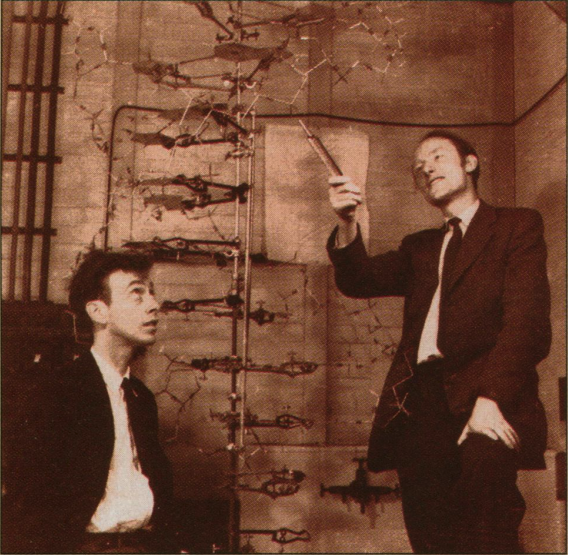
\includegraphics[width=0.6\columnwidth]{images/Watson_and_Crick.png}
   \caption{Watson and Crick frente al modelo de doble hélice. Fuente \cite{hallOldSchoolTies1993}}
   \label{fig:Watson_and_Crick}
\end{figure}
 
% 5
Casi al unísono, en 1953, otro importante descubrimiento fue publicado: la estructura del ADN \cite{watsonMolecularStructureNucleic1953}.
Usando cristalografía de rayos X James Watson and Francis Crick (figura \ref{fig:Watson_and_Crick}) establecieron que el ADN es un polímero con una conformación en doble hélice donde las bases nitrogenadas están apareadas por afinidad química.
Estos resultados sugerían que la información genética estaba codificada en la larga secuencia de esos pares.
Toda la diversidad de la vida ``escrita'' en un mismo lenguaje.
Había nacido la Genética Molecular.

% 5
También de relevante en ese período fue el trabajo de Frederick Sanger, quien publicó en 1951 la secuencia de una de las cadenas de la Insulina \cite{sangerAminoacidSequencePhenylalanyl1951}.
Estos resultados terminaron de imponer la teoría de que las proteínas son polímeros de aminoácidos con una secuencia lineal definida.
El vínculo entre la estructura de las proteínas y la secuencia de ADN era más evidente que nunca antes.
Comenzaban así a dibujarse los primeros bosetos del dogma central de la Biología Molecular.


\section{Segunda mitad del siglo XX}
 
Hasta ahora no hemos mencionado ningún ejemplo sobre el uso de la Computación en las investigaciones biológicas.
Esto tiene una explicación muy simple, durante la primera mitad del siglo XX el acceso a medios computacionales era escaso.
Como referencia, fue en 1946 que se terminó de construir la primera computadora electrónica de uso general, la ENIAC.
En estas etapas iniciales solo las instituciones más grandes (como los gobiernos y los ejércitos) tenían acceso a estas máquinas.
Pero a finales de los 50's esta tendencia fue cambiando, ya comenzaba a ser común para algunas universidades disponer de estos medios.
 
\begin{figure}[tb]
   \centering
   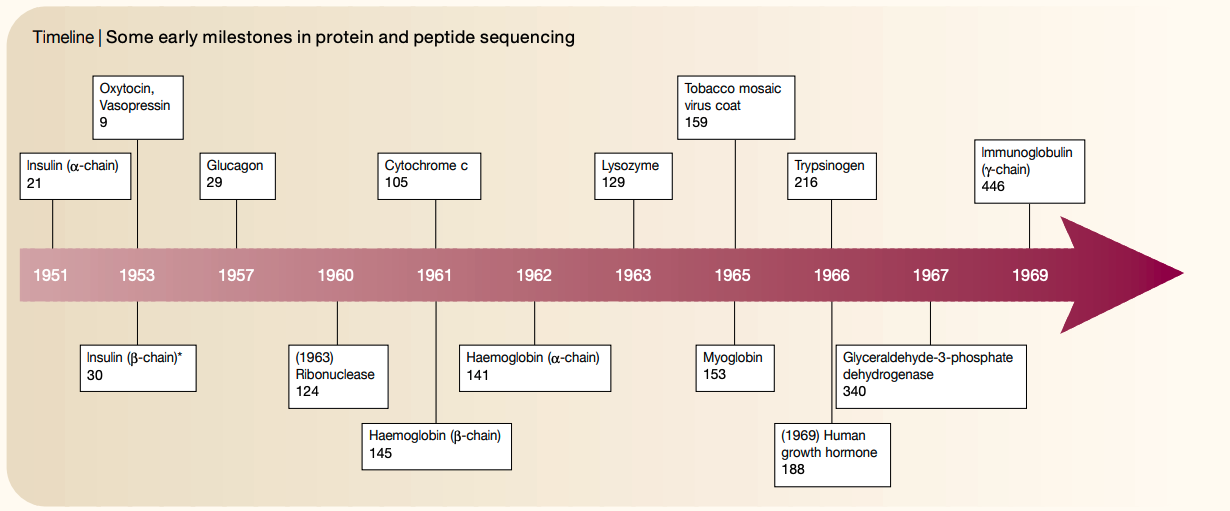
\includegraphics[width=1.0\columnwidth]{images/Protain_seq_milestones.png}
   \caption{
       (\textit{Figura en inglés})
       Momentos claves iniciales en el proceso de secuenciación de proteínas.
       Los números debajo de los nombres de las proteínas indican el número de aminoácidos de su secuencia (ej: Glucagón: 29).
       Fuente \cite{hagenOriginsBioinformatics2000}}
   \label{fig:Protain_seq_milestones}
\end{figure}
 
Mientras tanto, el primer enunciado formal del dogma central de la Biología Molecular fue expuesto por el propio Francis Crick durante una conferencia en 1957 \cite{cobb60YearsAgo2017}.
En este, las secuencias de ADN juegan el papel central como punto de partida del flujo de la información que caracteriza el desarrollo de los organismos.
A pesar de esto, por limitaciones experimentales de la época, son las secuencias proteicas las que son más accessibles.
Luego de que las primeras proteínas fueran resueltas ``a mano'', desde principios de los 60's se comienza a automatizar el proceso.
Proteínas cada vez más ``largas'' se secuenciaron en cada vez menos tiempo (figura \ref{fig:Protain_seq_milestones}).
A finales de los 60's, Pehr Edman diseñó el \textit{sequenator} \cite{edmanProteinSequenator1967}, un equipo completamente automático.
Cada vez más laboratorios se aventuraban a secuenciar proteínas de interés y así surgieron los primeros repositorios de secuencias \cite{hagenOriginsBioinformatics2000}.
 
\begin{figure}[h]
   \centering
   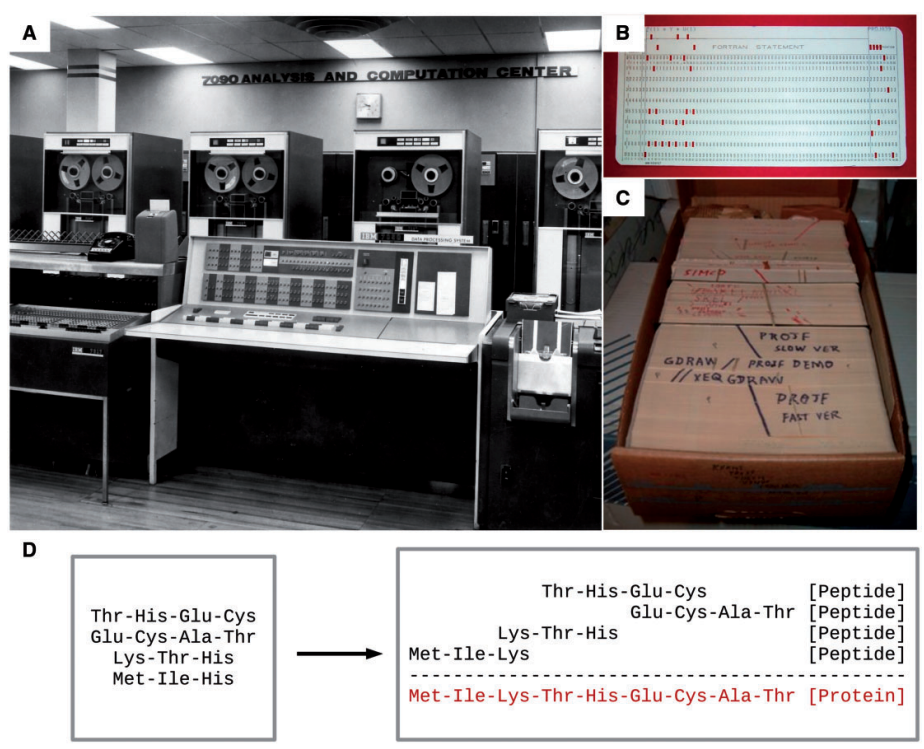
\includegraphics[width=0.7\columnwidth]{images/COMPROTEIN.png}
   \caption{
       Lo que es considerado como uno de los primeros sistemas bioinformáticos.
       \textbf{Panel A}: una computadora de la época (1962).
       \textbf{Panel B}: una tarjeta perforada (un medio de almacenamiento digital ``antiguo'').
       \textbf{Panel C}: conjunto de miles de tarjetas perforadas que contienen el programa ensamblador.
       \textbf{Panel D}: representación del proceso de ensamblaje de la secuencia completa a partir de los fragmentos secuenciados.
       Fuente \cite{gauthierBriefHistoryBioinformatics2019}}
   \label{fig:COMPROTEIN}
\end{figure}
 
% 5
El uso de las computadoras durante el proceso de secuenciación fue imprescindible desde bien temprano (figura \ref{fig:COMPROTEIN}) \cite{dayhoffAComputerProgram1962}.
El problema principal radicaba en que los métodos bioquímicos de la época solo podían resolver en cada corrida secuencias de tamaño limitado.
Por ello, para secuenciar proteínas de mayor tamaño, estas eran divididas en fragmentos manejables que se procesaban individualmente.
Luego, la secuencia completa de la proteína era reconstruida aprovechando secciones redundantes entre los fragmentos adyacentes.
La complejidad del proceso reconstructivo aumenta considerablemente con el tamaño de las proteínas y la cantidad de fragmentos en cuestión, por lo que rápidamente se hace impráctico realizarlo manualmente.

%  5
Los años 50's y 60's son etapas muy tempranas en el desarrollo de la Computación.
El hecho de que ya desde esta época la Biología asimilara su uso pone de manifiesto un patrón universal en la ciencia.
No existen herramientas únicas de un campo o disciplina, o herramientas que no sean de su interés.
Esas ideas son, en el mejor de los casos, solo una ilusión temporal.
Lo que existen son problemas, cuestiones que se quieren resolver.
El cómo atacarlos cambia dependiendo de qué recursos estén disponibles.
Seguramente Albert Eistein no estudió programación en la universidad (las computadoras no eran muy populares por esa época), sin embargo, pero al tiempo de su muerte en 1955, los físicos ya habían incorporado esta a su caja de herramientas.

% 5
Sin embargo, el impacto del uso de la Computación en las investigaciones biológicas solo comenzaba.
La acumulación de secuencias de proteínas potenció el desarrollo de nuevas ramas dentro de esta ciencia.
Una de las más tempranas fue el campo de la Evolución Molecular.
El dogma central tiene consecuencias muy interesantes.
Primero, al ser el ADN el principal portador de la información genética, la evolución puede ser vista como la acumulación de cambios en dicha secuencia y su posterior discriminación por seleción natural.
De esta manera, una comparación de secuencias de diferentes especies debería arrojar luz sobre su pasado evolutivo.
Segundo, que se puede aprender sobre las secuencias de ADN partiendo del estudio de las secuencias de las proteínas.
Así, los estudios evolutivos también se podían llevar a cabo empleando las secuencias de estas últimas.
 
\begin{figure}[h]
   \centering
   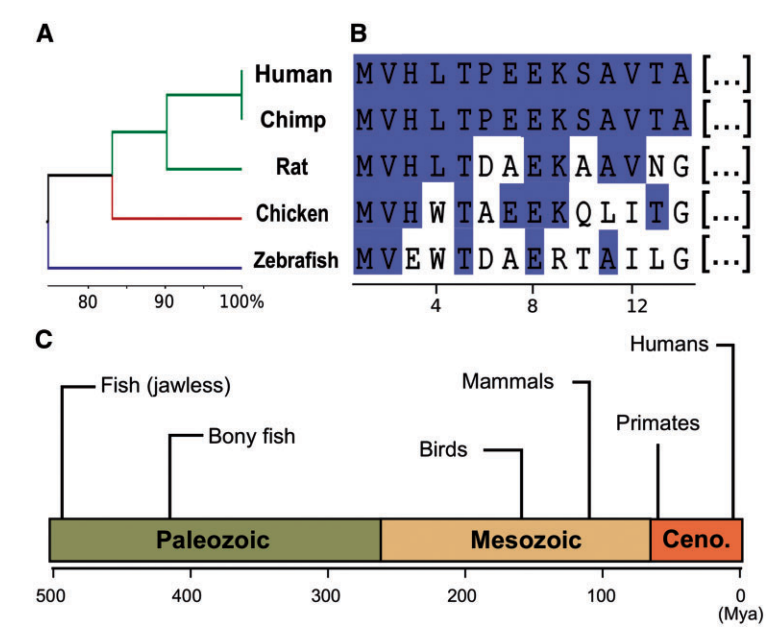
\includegraphics[width=0.7\columnwidth]{images/evolution.png}
   \caption{
       (\textit{Figura en inglés})
       \textbf{Panel A y B}: el árbol filogenético (izquierda) y un fragmento de la comparación (derecha) entre las secuencias de hemoglobina que se emplearon en su elaboración (cada letra representa un aminoácido).
       \textbf{Panel C}: cronología de los fósiles más antiguos encontrados de las especies/grupos estudiados (\textit{Mya} Millones de años).
       Fuente \cite{gauthierBriefHistoryBioinformatics2019}}
   \label{fig:evolution}
\end{figure}

% 5
La hipótesis era simple.
Si dos especies divergieron recientemente en la historia evolutiva, las secuencias de proteínas comunes a ambas (denominadas homólogas) deberían ser similares.
Por el contrario, si las especies están muy poco emparentadas, esta similitud se espera sea menor.
De esa forma, ordenando un grupo de especies con respecto a la ``similitud'' entre sus secuencias homólogas, se podría construir su árbol filogenético.
Por ejemplo, si se compara la secuencia de la hemoglobina humana con la del chimpancé se aprecian menos diferencias que entre un humano y un ratón.
Los árboles filogenéticos obtenidos de esta forma fueron luego comparados,  con muy buenos resultados, con los obtenidos mediante los métodos tradicionales, como el registro fósil (figura \ref{fig:evolution}) \cite{fitchConstructionPhylogeneticTrees1967}.

% 5
Una vez más, la Computación fue clave en estas investigaciones.
Mientras más secuencias de más especies se acumulaban, realizar el alineamiento necesario para determinar su similitud se hacía demandante, incluso, para las computadoras más avanzadas;
sobre todo si las especies estudiadas estaban muy poco emparentadas y las diferencias entre las secuencias eran pronunciadas o implicaban adiciones o eliminaciones.
Como referencia, comparar solo $10$ secuencias de $100$ aminoácidos de extensión cada una tomaba como promedio $10^{18}$ operaciones \cite{wangComplexityMultipleSequence1994}.
Estas investigaciones no solo estaban en la vanguardia de la Biología, sino también de la Computación.
Como veremos a continuación esta tendencia llega hasta hoy día.
La relación entre ambas ciencias siempre ha sido de beneficio mutuo y con una clara inclinación a profundizarse.


\section{Años 90's: Despegue de las ómicas}

Aunque las secuencias de proteínas fueron un punto de partida dada su temprana disponibilidad, la secuenciación de ADN también fue avanzando aceleradamente y ya en la década de los 90's tenía gran desarrollo.
Ejemplo de esto fue la secuenciación del primer genoma completo de un organismo independiente (no parásito) en 1995, \textit{Haemophilus influenzae} \cite{fleischmannWholegenomeRandomSequencing1995}.
Pero aún más importante fue el lanzamiento de unos de los proyectos más ambiciosos en la historia de Biología: el Proyecto del Genoma Humano.

\begin{figure}[tb]
  \centering
  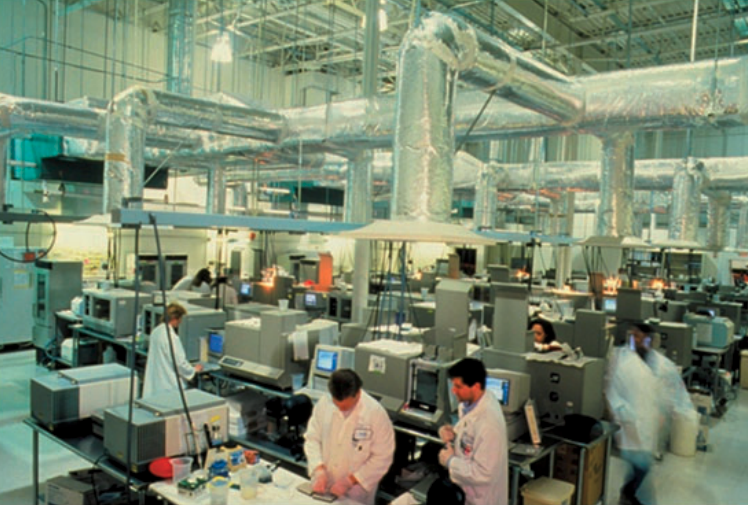
\includegraphics[width=0.7\columnwidth]{images/human_genome_project.png}
  \caption{Secuenciación a escala industrial durante Proyecto del Genoma Humano. Fuente \cite{gauthierBriefHistoryBioinformatics2019}}
  \label{fig:human_genome_project}
\end{figure}

El proyecto, financiado principalmente por el gobierno de los Estados Unidos, comenzó en 1991 (figura \ref{fig:human_genome_project}).
Una década, 2.7 miles de millones de dólares y 3 mil millones de pares de bases después \cite{web:HGP_FAQ}, se presentaba la primera versión de un genoma humano de referencia \cite{internationalhumangenomesequencingconsortiumFinishingEuchromaticSequence2004}.
Este acontecimiento es considerado el punto de partida de lo que se conoce como la era de las \textit{ómicas} en la Biología.

Las ómicas son un conjunto de disciplinas que se especializan en el estudio de los componentes o relaciones que conforman un organismo vivo (figura \ref{fig:Central_Dogma}).
Estas disciplinas se caracterizan por su carácter total, no se estudia un componente en particular, se intenta alcanzar a todos en el organismo en cuestión.
Entre ellas están las que estudian los diferentes componentes moleculares, la genómica (el ADN), la transcriptómica (el ARN), la proteómica (las proteínas), la metabolómica (los intermediarios metabólicos), etc.
Además están las que estudian otros aspectos como la epigenética (estudio de los patrones de metilación del ADN), la fenómica (estudio de todos los fenotipos mutantes), la regulómica (los componentes moleculares regulatorios) y muchas más \cite{evansDesignerScienceOmic2000}.
El patrón es simple, ``algo biológicamente interesante'' + ``ómica''.
Estas, casi siempre surgen cuando se desarrolla alguna técnica experimental que permite obtener los datos requeridos a gran escala.

\begin{figure}[tb]
  \centering
  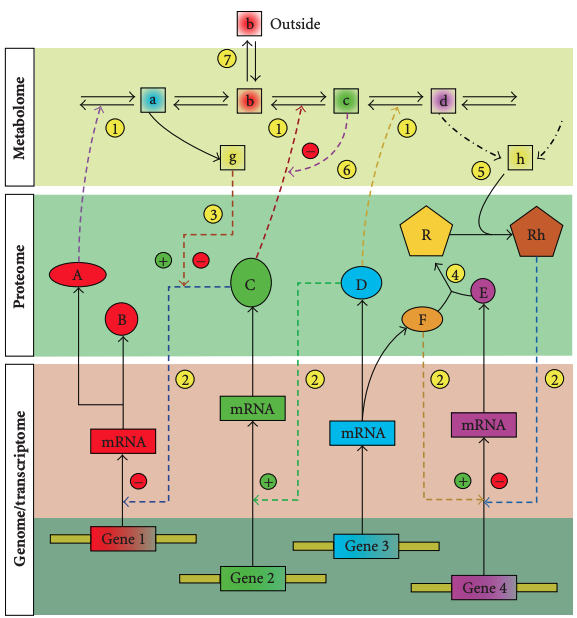
\includegraphics[width=0.7\columnwidth]{images/Central_Dogma.png}
  \caption{
      (\textit{Figura en inglés})
      El Dogma Central de la Biología Molecular y las ómicas.
      Con el desarrollo de las ómicas se pretende construir un mapa detallado que comprenda todos los componentes celulares y sus interrelaciones, cientos de miles de componentes y millones de interacciones.
      Fuente \cite{likicSystemsBiologyNext2010a}}
  \label{fig:Central_Dogma}
\end{figure}

En estas disciplinas los conceptos computacionales no son solo fundamentales, sino nativos.
Junto con los elaborados procedimientos experimentales, nuevas tecnologías y algoritmos deben ser creados para hacer frente a la cantidad de datos sin precedentes que se generan.
Un papel muy importante en las etapa inicial de desarrollo de las ómicas lo jugó la evolución de la red mundial de computadoras \cite{gauthierBriefHistoryBioinformatics2019}.
A principios de los 90's Tim Berners-Lee crea la \textit{World Wide Web}, un sistema internacional de documentos interconectados, lo que se considera como el comienzo de la internet \cite{web:WWW}.
Esta red ha jugado, y juega, un papel esencial a la hora de facilitar la colaboración a gran escala necesaria en proyectos de gran magnitud.
Desde el almacenamiento hasta la publicación y acceso de los resultados, la Biología es ``subida a la nube''.



\section{Siglo XXI}

\begin{figure}[tb]
  \centering
  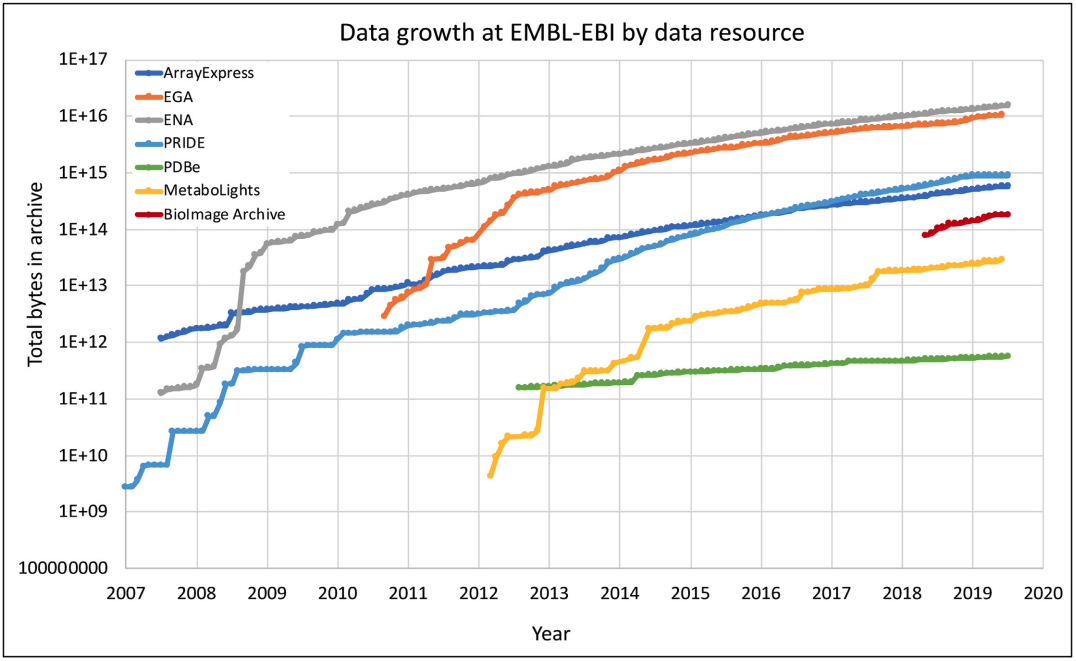
\includegraphics[width=0.9\columnwidth]{images/Dat_trend.png}
  \caption{
      (\textit{Figura en inglés})
      Crecimiento exponencial de los datos manejados por el Instituto Europeo de Bioinformática (EMBL-EBI).
      Note que un Terabyte son $10^{12}$ bytes.
      En la gráfica se muestra la evolución de diferentes bases de datos, desde genómicas hasta imágenes de microscopía.
      Para más detalles ir a la Fuente \cite{cookEuropeanBioinformaticsInstitute2020}
  }
  \label{fig:Dat_trend}
\end{figure}

En las últimas dos décadas la Biología se ha posicionado como una de las ciencias que genera mayor cantidad de datos.
Por ejemplo, en el 2015, la cantidad de genomas humanos secuenciados se duplicaba cada 7 meses.
O sea, si a comienzos de los 2000 tras una década de trabajo se publicaba el primer genoma humano, veinte años después se acumulan más de un millón.
¿Y es eso mucho?
Como referencia tomen que, en 2015, \textit{youtube} generó entre 1-2 exabytes (millones de terabytes) de nuevo contenido, mientras que se estima que la genómica como campo pudo generar hasta 40 \cite{stephensBigDataAstronomical2015}.
Esta tendencia no es única para la genómica.
Cada elemento de interés biológico está siendo estudiado y recopilado en enormes bases de datos.
¡Hay curvas de crecimiento exponencial por todos lados! (figura \ref{fig:Dat_trend}).

A pesar de esto, aunque es un gran reto, el almacenamiento no es el mayor de los problemas a enfrentar en la actualidad.
Más agudo aún es el de extraer de los datos la información relevante.
Por ejemplo, si reevaluamos el alineamiento de secuencias en el contexto contemporáneo veremos la magnitud del reto.
El alineamiento de un genoma completo de humano con otro de ratón, usando los últimos algoritmos, toma alrededor de 100 horas ($\sim$ 4 días) en un CPU moderno.
Ahora, si escalamos este análisis para todos los genomas de las más de 2.5 millones de especies que se espera tener secuenciadas para el 2025, se necesitaría toda la capacidad actual de cómputo de la humanidad multiplicada por un millón \cite{stephensBigDataAstronomical2015}.
¿Pero acaso la humanidad no está aumentando su poder de cómputo exponencialmente? ¿No se puede simplemente esperar hasta que sea suficiente?
Pues no es tan simple, mientras que la evolución del poder de cómputo ha seguido la tendencia de duplicarse cada 2 años (llamada Ley de Moore), incluso aunque esta se mantenga, la generación de datos biológicos es simplemente mucho mayor (es duplicada en menos de un año) \cite{stephensBigDataAstronomical2015}.
A esto se le suma el hecho de que hay otras áreas de la actividad humana generando cantidades similares de datos, desde la Astrofísica hasta las redes sociales.
No todas las computadoras son para nosotros.

La discusión anterior ilustra sólo una parte del problema: el enorme volumen de datos dificulta incluso la aplicación de técnicas ya establecidas.
Pero otro igual de significativo es el de generar nuevas formas de análisis.
Por ejemplo, en la era pre-ómicas, las áreas de la Biología que intentaban construir modelos detallados de sistemas completos no atraían mucho interés.
Los sistemas vivos son simplemente demasiado complejos.
Estos pueden comprender miles de componentes por cada célula, miles de tipos celulares por cada organismo y un sin número de especies diferentes por ecosistema.
Todo ello extremadamente interconectado y sometido a cambios constantes.
Sin los datos suficientes, la creación de modelos capaces de capturar tal complejidad estaba fuera del alcance de los investigadores.
Pero en los últimos años la situación es diferente, como se evidencia con la consolidación de la Biología de Sistemas \cite{likicSystemsBiologyNext2010a}.
Esta disciplina intenta explicar detalladamente la relación que enuncia el dogma central y sus consecuencias:
¿cómo el genoma determina función?
Este nuevo enfoque mueve el centro de estudio desde el \textit{elemento} a la \textit{red de elementos}.
O sea, se trata de explicar cómo una determinada función emerge de la interacción de las partes del sistema.
Lo cual es posible  solo si se tienen datos lo suficientemente completos para representar una parte significativa del mismo.

\begin{figure}[tb]
  \centering
  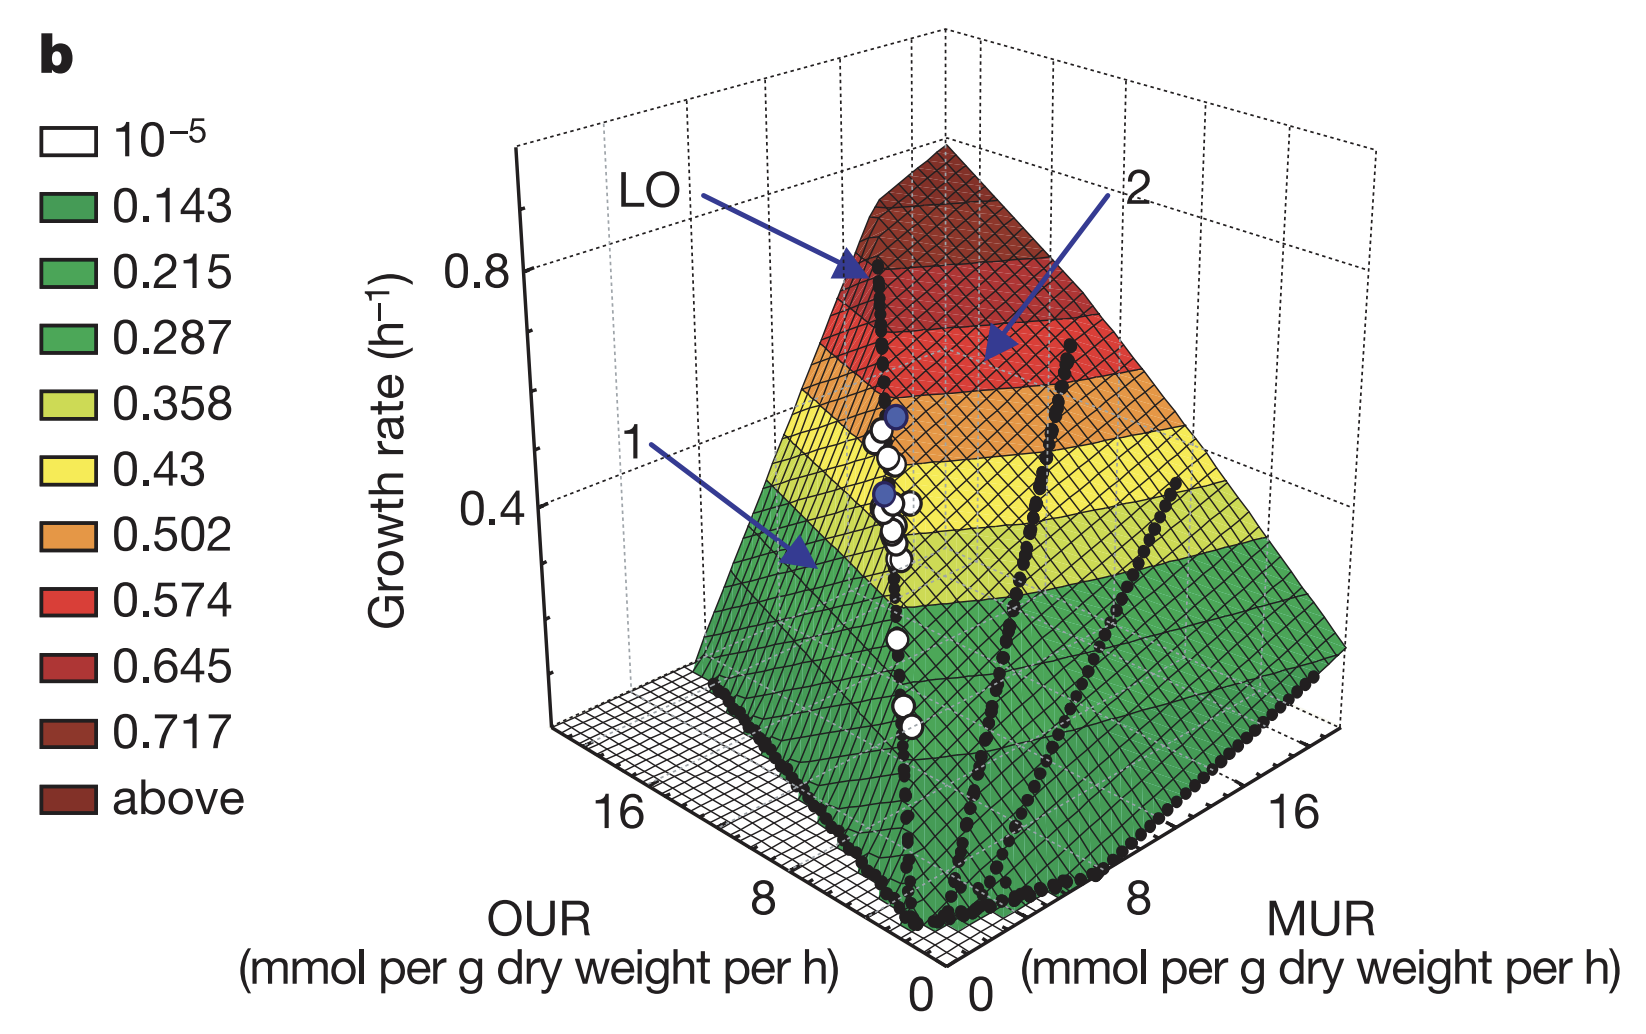
\includegraphics[width=0.9\columnwidth]{images/Ecoli_growth.png}
  \caption{
      (\textit{Figura en inglés})
      En la figura se muestra cómo dadas las disponibilidades de malato (MUR) y oxígeno (OUR), principales nutrientes limitantes en el cultivo, el crecimiento de la bacteria (círculos blancos y azules) sigue la tendencia esperada descrita por el modelo (puntos negros).
      Para más detalles ir a \cite{ibarraEscherichiaColiK122002}
  }
  \label{fig:Ecoli_growth}
\end{figure}

Por ejemplo, hoy se dispone de redes que comprenden todas las reacciones metabólicas que se han identificado en el genoma de $\textit{Escherichia coli}$.
Con estas redes se pueden construir modelos para simular el crecimiento de dicha bacteria en un medio dado.
A medida que más datos se le han ido incorporando a estos modelos, estos han ido mejorando su poder predictivo \cite{ibarraEscherichiaColiK122002}.
Además de las aplicaciones ingenieriles que se pueden derivar, la modelación también contribuye a generar conocimientos biológicos.
En los resultados mostrados en la figura \ref{fig:Ecoli_growth}, por ejemplo, los valores experimentales (círculos blancos y azules) se ubican en el máximo posible dada las restricciones que establece el modelo.
O sea, las bacterias están creciendo tanto como pueden dada la disponibilidad de nutrientes y su capacidad metabólica, lo cual pudiera ser referente de la presión adaptativa a la que se enfrentan típicamente en su ambiente natural.
En general, avances como este hacen que la Biología se mueva cada vez más de su enfoque experimental de ``prueba y error'' a otro mucho más teóricamente intenso.

Por otro lado, la disponibilidad de grandes cantidades de datos sin analizar no ha pasado inadvertida por otras disciplinas.
Físicos, ingenieros, científicos de la Computación y muchos otros especialistas están tratando de modificar las técnicas y habilidades que emplean en sus campos para analizar los datos biológicos.
Un ejemplo reciente es el caso de \textit{DeepMind}, una subsidiaria de \textit{google}.
Anteriormente, en el año 2017, esta empresa de inteligencia artificial logró el hito de crear un programa para jugar \textit{Go} que pudo vencer al jugador humano con el primer puesto en el ranking de ese deporte.
Pero en el año 2020, \textit{DeepMind} volvió a ser noticia.
Esta vez fue por usar su enorme capacidad para atacar lo que es considerado uno de los problemas computacionales más grandes de la Biología: predecir la estructura 3D de las proteínas a partir de su secuencia lineal \cite{callawayItWillChange2020}.
En particular, \textit{DeepMind} sobrepasó a otros 100 equipos en un concurso bianual llamado $\textit{CAPS}$.
En este concurso alrededor de 100 secuencias de proteínas son publicadas.
Las estructuras 3D de estas proteínas son determinadas a partir de técnicas experimentales ya establecidas pero esta información no es pública hasta después del concurso.
Así, los equipos tienen dos años para proponer sus propias estructuras que luego son comparadas con las experimentales.
El uso masivo por parte de $\textit{DeepMind}$ de nuevas técnicas de $\textit{Machine Learning}$ les permitió obtener resultados revolucionarios en esta área (figura \ref{fig:Deep_Mind}) \cite{callawayItWillChange2020}.
 
\begin{figure}[tb]
  \centering
  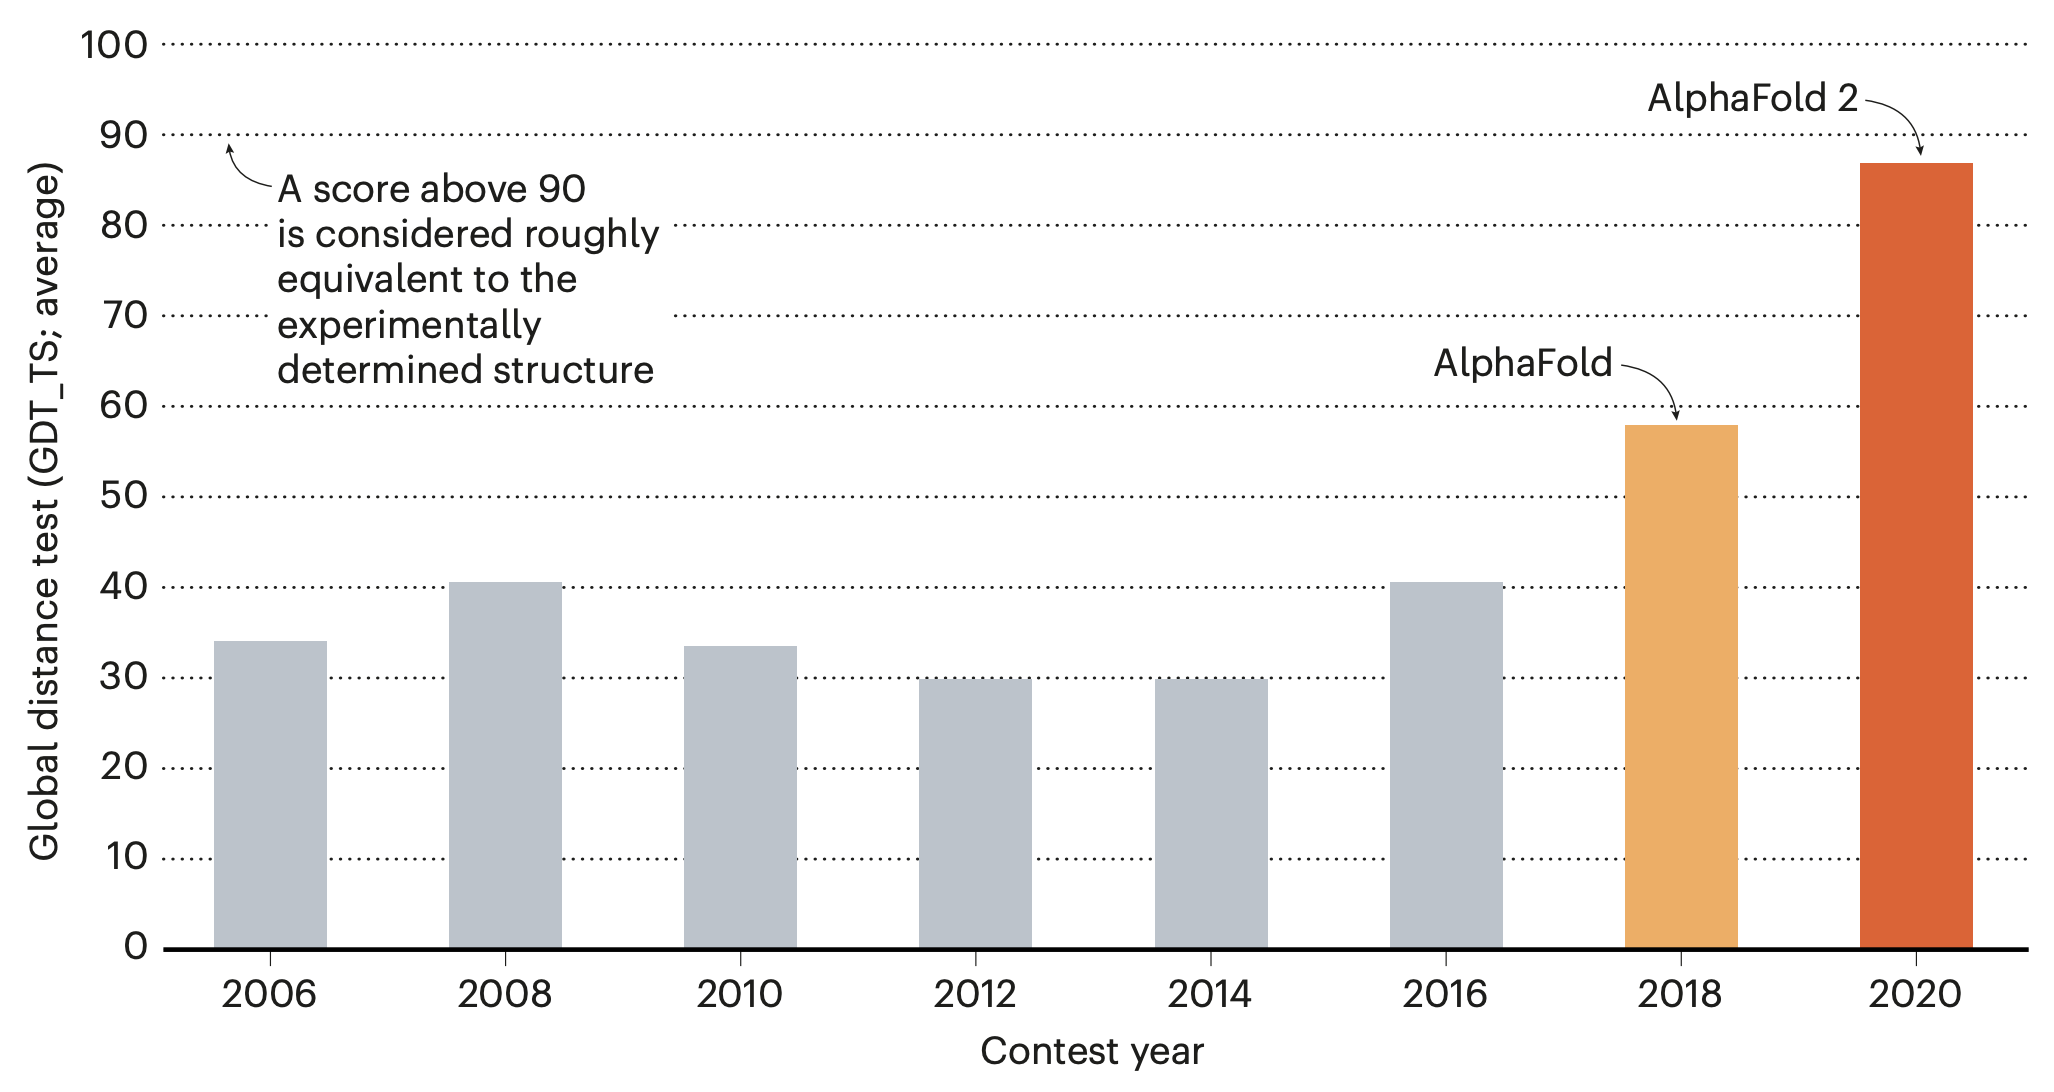
\includegraphics[width=0.9\columnwidth]{images/Deep_Mind.png}
  \caption{
      (\textit{Figura en inglés})
      $\textit{AlphaFold}$, las redes de $\textit{DeepMind}$, han revolucionado el campo de la predicción de la estructura 3D de las proteínas a partir de su secuencia lineal.
      Sus predicciones están cerca de tener un 90\% de similitud con los resultados experimentales.
      Fuente \cite{callawayItWillChange2020}
  }
  \label{fig:Deep_Mind}
\end{figure} 

 



\section{Biología ``quo Vadis'' \texorpdfstring{$^\dagger$}{}}
 
\let\thefootnote\relax\footnotetext{$\dagger$ \textit{quo Vadis}: del latín ``¿A dónde vas?''}
\begin{figure}[tb]
  \centering
  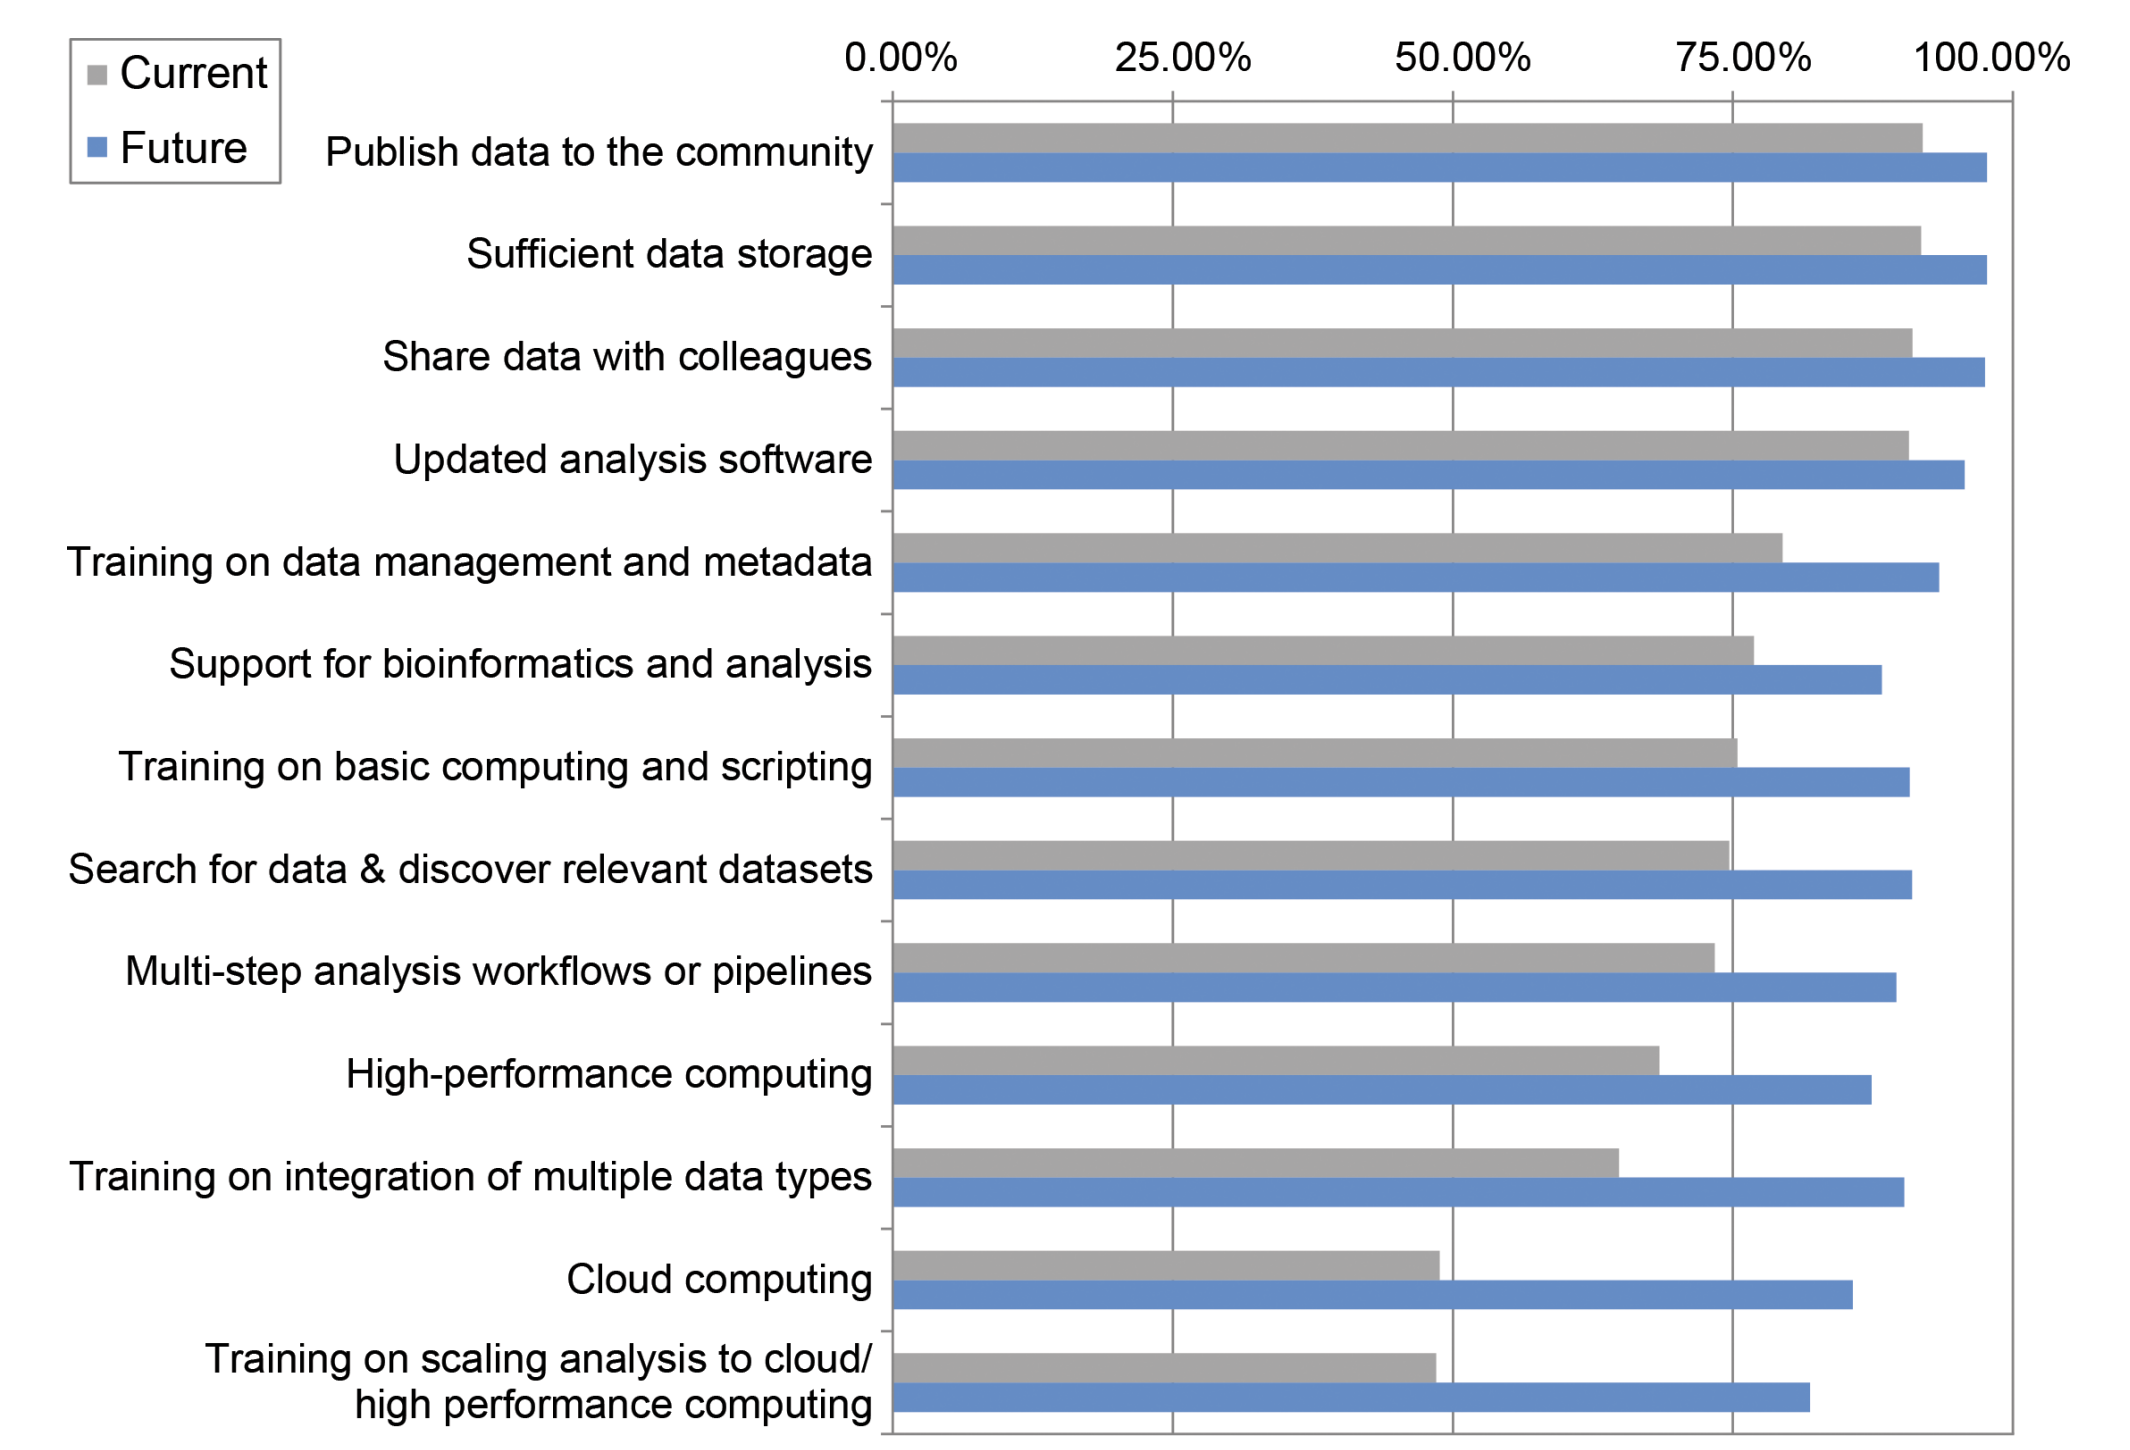
\includegraphics[width=0.8\columnwidth]{images/survey.png}
  \caption{
      (\textit{Figura en inglés})
      Necesidades computacionales actuales y futuras identificadas en una encuesta realizada a cientos de investigadores.
      Noten que las necesidades futuras son siempre mayores que las actuales, en algunos casos marcadamente.
      Fuente \cite{baroneUnmetNeedsAnalyzing2017}}
  \label{fig:survey}
\end{figure}
 
Como se mencionó al comienzo, es imposible abarcar en un documento tan breve el desarrollo de una ciencia tan amplia como la Biología.
Por ello, inevitablemente, se han quedado fuera muchas otras disciplinas que son ejemplos de la profunda interrelación entre la Computación y esta rama de la ciencia.
Entre ellas podemos mencionar a las Neurociencias, la Biología Celular, la Fisiología, la Ecología y otras que se han beneficiado, por ejemplo, del desarrollo de las tecnologías de imágenes digitales y su procesamiento.
Desde imágenes satelitales que son empleadas para evaluar la progresión de un daño ecológico o los patrones de migración de especies amenazadas \cite{kwokEcologyRemotesensingRevolution2018}, hasta el entrenamiento de redes neuronales para el temprano diagnóstico de cáncer a partir de imágenes de muestras de tejido \cite{mohammadzadehAdvancesOptimalDetection2015}.
Otras como la Bioacústica y la Biofísica se han beneficiado grandemente del desarrollo del procesamiento de señales en general.
Por ejemplo, investigadores graban el sonido ambiente en los hábitats y luego lo procesan para estimar simultáneamente el tamaño de poblaciones de diversas especies.
La identificación y el conteo de los individuos se puede realizar mediante \textit{Machine Learning} \cite{kahlBirdNETDeepLearning2021}.
Al igual que las ómicas, todas estas disciplinas vienen acompañada de grandes acumulaciones de datos.
 
Por otro lado, otro fenómeno significativo es la democratización del acceso a las tecnologías de la información.
Movimientos como el $\textit{Open Software}$ y $\textit{Open Hardware}$ han abierto un sinfín de nuevas posibilidades \cite{ravindranHowDIYTechnologies2020}, particularmente en los países en vías de desarrollo.
Hoy en día es posible fabricar ``en casa'', usando tecnologías como la impresión 3D y microcontroladores, los sensores e instrumentos necesarios para la investigación.
Esto no solo puede abaratar los costos, también permite que los investigadores diseñen los artefactos acorde a sus necesidades más particulares.
Nunca ha habido más flexibilidad en el aspecto experimental.

La Biología se encuentra hoy en una posición muy diferente si es comparada con los comienzos de este siglo.
La disponibilidad de grandes cantidades de datos ha aumentado considerablemente la necesidad de introducir nuevas habilidades en el currículum de los estudiantes e investigadores.
En una encuesta reciente realizada a varios cientos de investigadores de alto perfíl, se identificó como una de las principales áreas a priorizar, el entrenamiento de las nuevas generaciones en las habilidades requeridas para la manipulación, publicación y procesamiento de datos \cite{baroneUnmetNeedsAnalyzing2017} (figura \ref{fig:survey}).
Esto avizora un futuro donde un sólido entrenamiento en computación no sea ya una habilidad excepcional, sino, esperada para un graduado de una especialidad biológica.
Como mencionamos anteriormente, no existen herramientas propias de una disciplina, ni herramientas que estén fuera de su interés. Existen problemas fundamentales, y cada disciplina deberá considerar suyas todas aquellas que les permitan abordar los propios, la Biología no es excepción.
 
\rightline{$\blacksquare$}
 


 
%----------------------------------------------------------------------------------------
%	BIBLIOGRAPHY
%----------------------------------------------------------------------------------------

% \newpage
\bibliographystyle{unsrt}

\bibliography{Computation_and_Biology.bib} % The file containing the bibliography

%----------------------------------------------------------------------------------------

\end{document}